
%%%%%%%%% BODY TEXT
\vspace{-5mm}
\section{Introduction}
\label{sec:intro}


%--------------------------------------------------------------------------------
\begin{figure}[!t]
% \vspace{-0.5cm}
    %\centering
    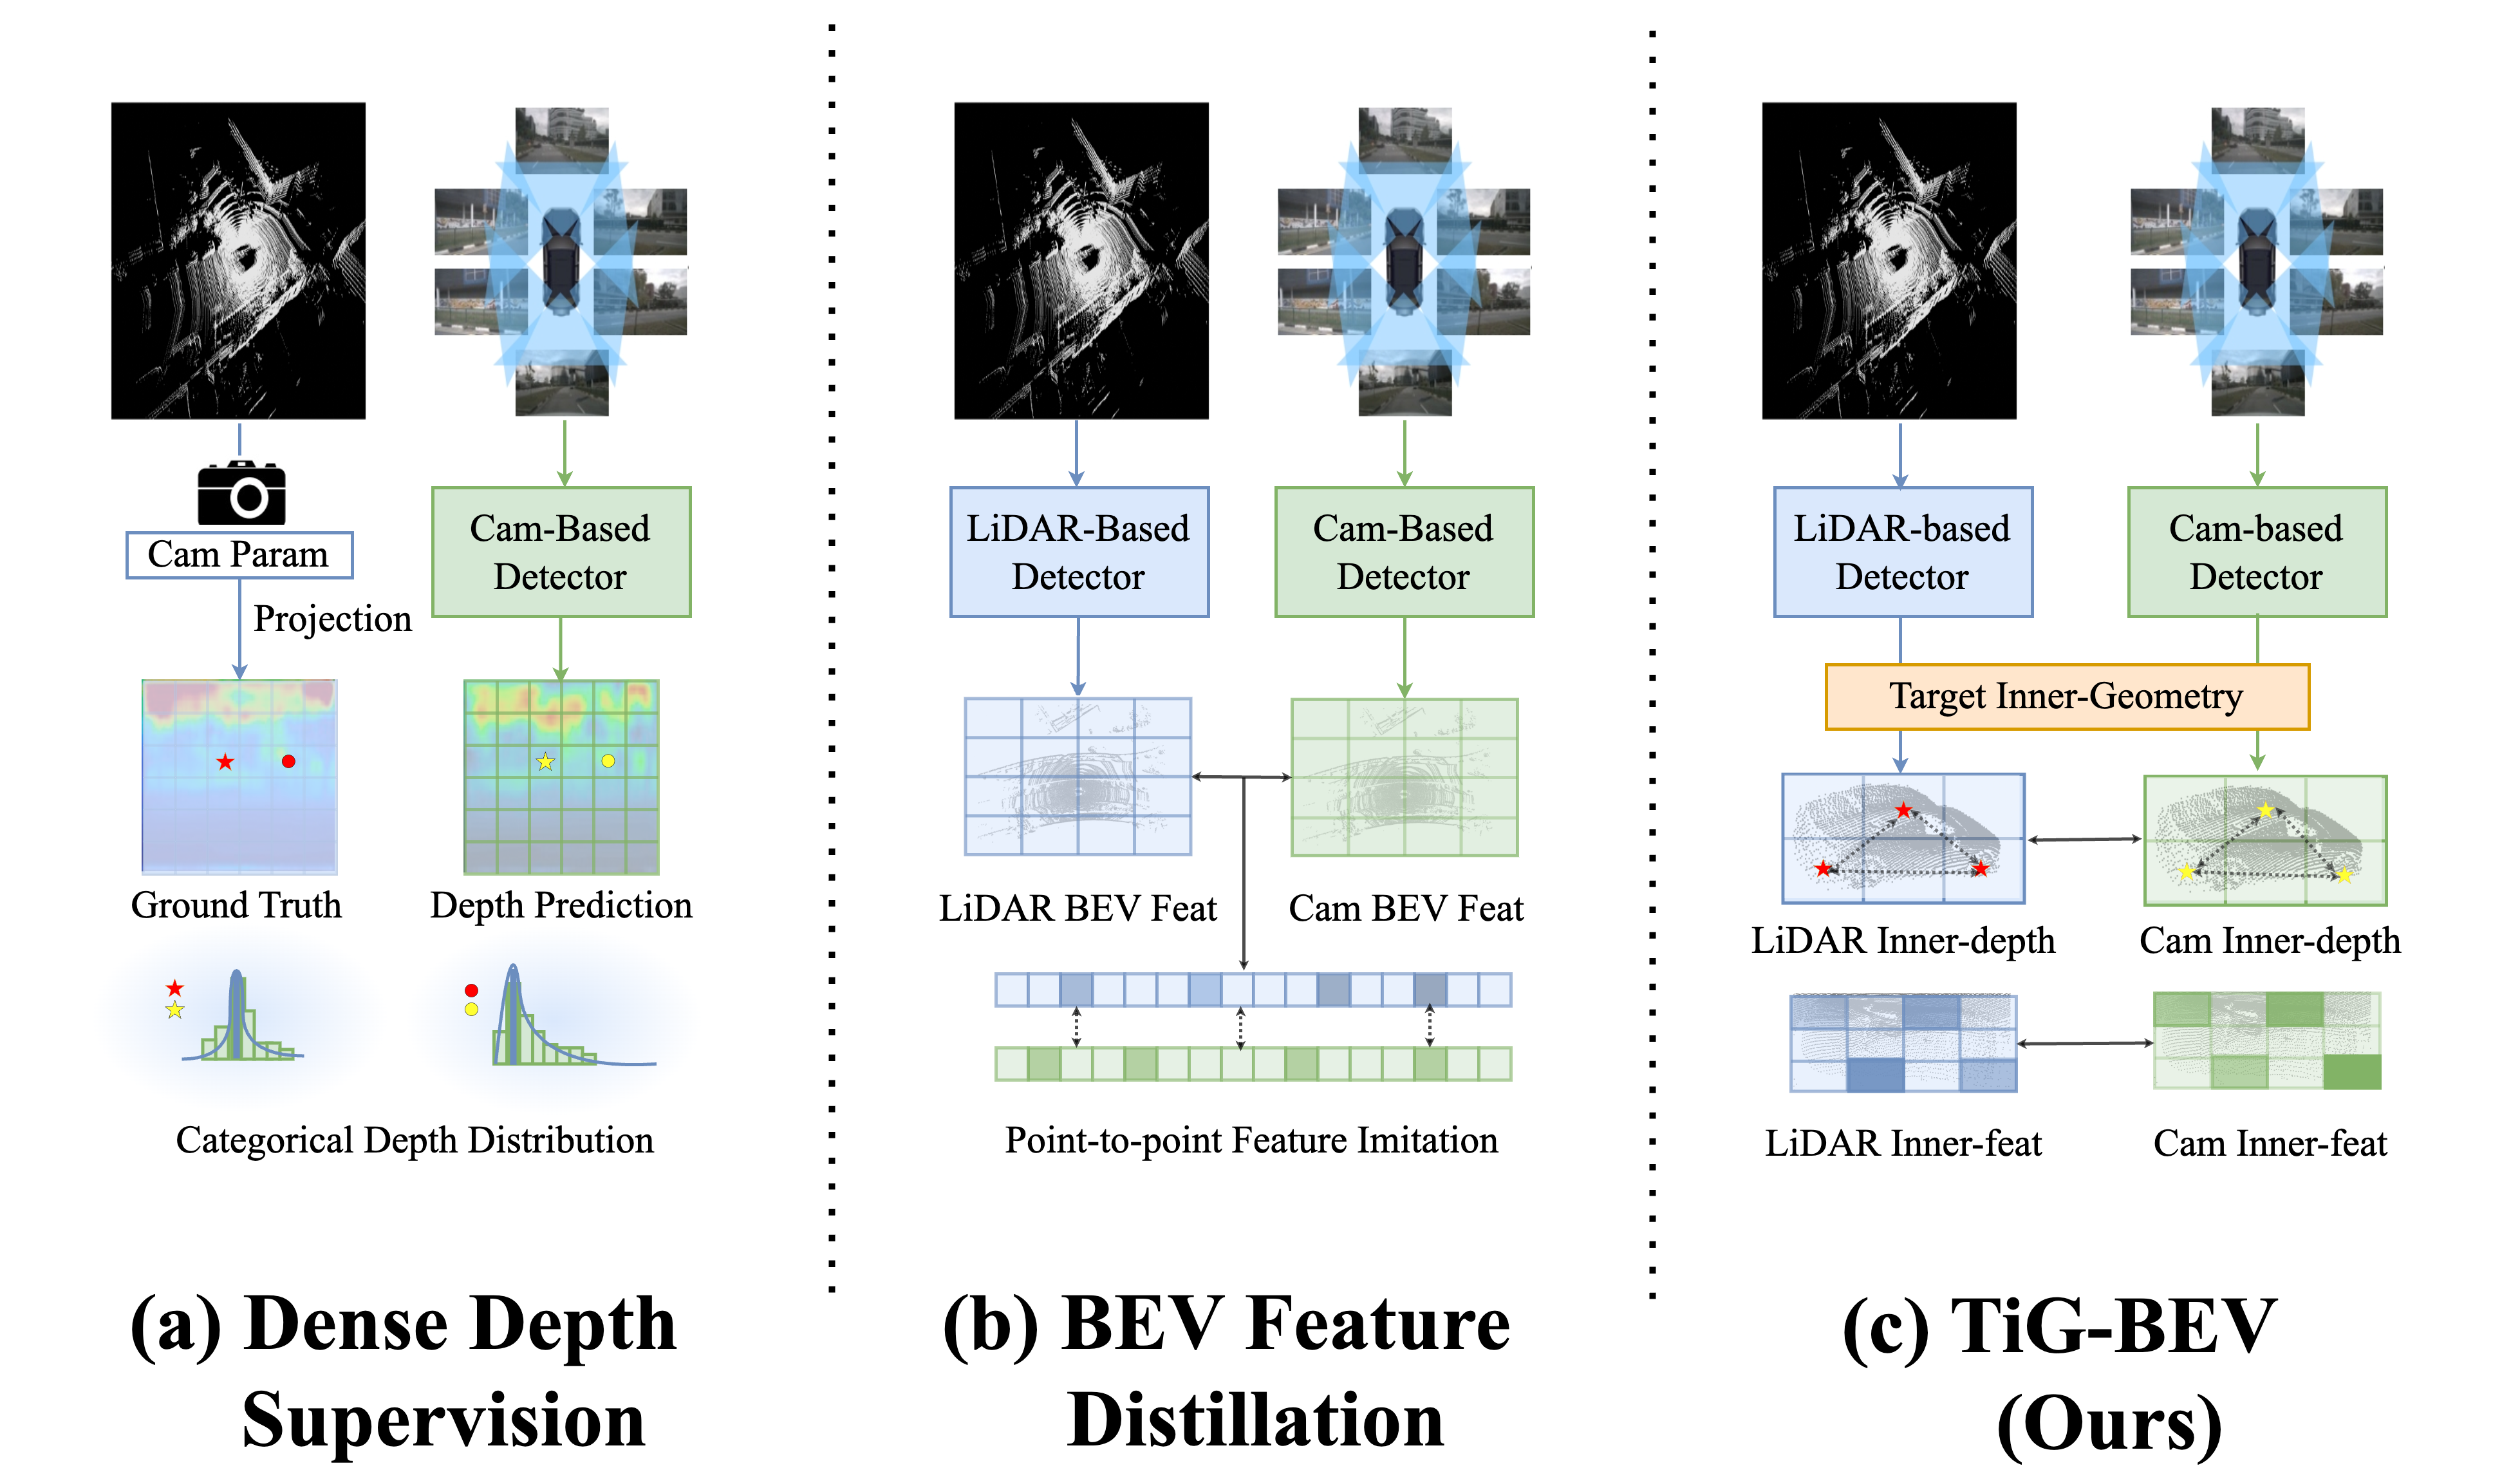
\includegraphics[scale=0.062]{cvpr_2022/iccv_fig1.drawio.png}
    % \vspace{0.5pt}
    \caption{\textbf{Different LiDAR-to-Camera Learning Schemes:} (a) Dense Depth Supervision~\cite{b7,b51}, (b) BEV Feature Distillation~\cite{b9,b52}, (c) Our Target Inner-Geometry Learning (TiG-BEV).
    }
    \label{fig:teaser_figure}
    % \vspace{-0.8cm}
\end{figure}

3D object detection aims to recognize and localize objects in 3D space, which is more challenging than its 2D counterpart and has achieved outstanding progress in various applications, such as robotics \cite{b1}, virtual reality \cite{b2}, and autonomous driving \cite{b3,b4,b5,b6}. Mainstream methods for 3D object detection can be categorized into LiDAR-based detectors \cite{b14, b3, b15} and camera-based detectors \cite{b7, b11, b12, b13, b47,b48}. Therein, LiDAR-based methods have attained excellent performance by taking 3D point clouds as input, which inherently contains sufficient spatial structures for accurate object localization. In contrast, camera-based methods are relatively low-cost with colored context information, but are constrained by the lack of geometric depth cues.

Considering the performance gap between camera-based and LiDAR-based detectors, 
existing methods leverage the spatial cues provided by the LiDAR modality to improve the accuracy of camera-based detectors, which are mainly in two schemes shown in Figure~\ref{fig:teaser_figure}. (1) Dense Depth Supervision (Figure~\ref{fig:teaser_figure} (a)), e.g., CaDDN~\cite{b51} and BEVDepth~\cite{b7}. These methods first project the input LiDAR points onto image planes using intrinsic and extrinsic camera parameters. Then, these derived depth maps are applied to explicitly supervise the categorical depth prediction within both foreground and background areas. (2) BEV Feature Distillation (Figure~\ref{fig:teaser_figure} (b)), e.g., CMKD~\cite{b52} and BEVDistill \cite{b9}. There methods adopt the teacher-student paradigm for BEV feature distillation. They force the BEV representation generated by the camera-based detector (student) to imitate that produced by a pre-trained LiDAR-based detector (teacher). By directly mimicking the BEV features, the student is expected to inherit the encoded high-level BEV semantics from the teacher.

However, existing methods fail to capture the inner-geometric characteristics of different foreground targets, i.e., the spatial contours and part-wise semantic relations. As examples, BEVDepth simply adopts pixel-by-pixel depth supervision without specializing the relative depth within objects, and BEVDistill applies foreground-guided distillation but neglects the inner relations of BEV features. In addition, methods~\cite{b9,b52} for BEV feature distillation directly enforce the channel-by-channel alignment between cross-modal BEV representations. Such strict mimicking might adversely affect the performance due to the modal gap between camera and LiDAR BEV features, i.e., visual appearances vs. spatial geometries.

\begin{figure}[!t]
\vspace{0.1cm}
    \centering
    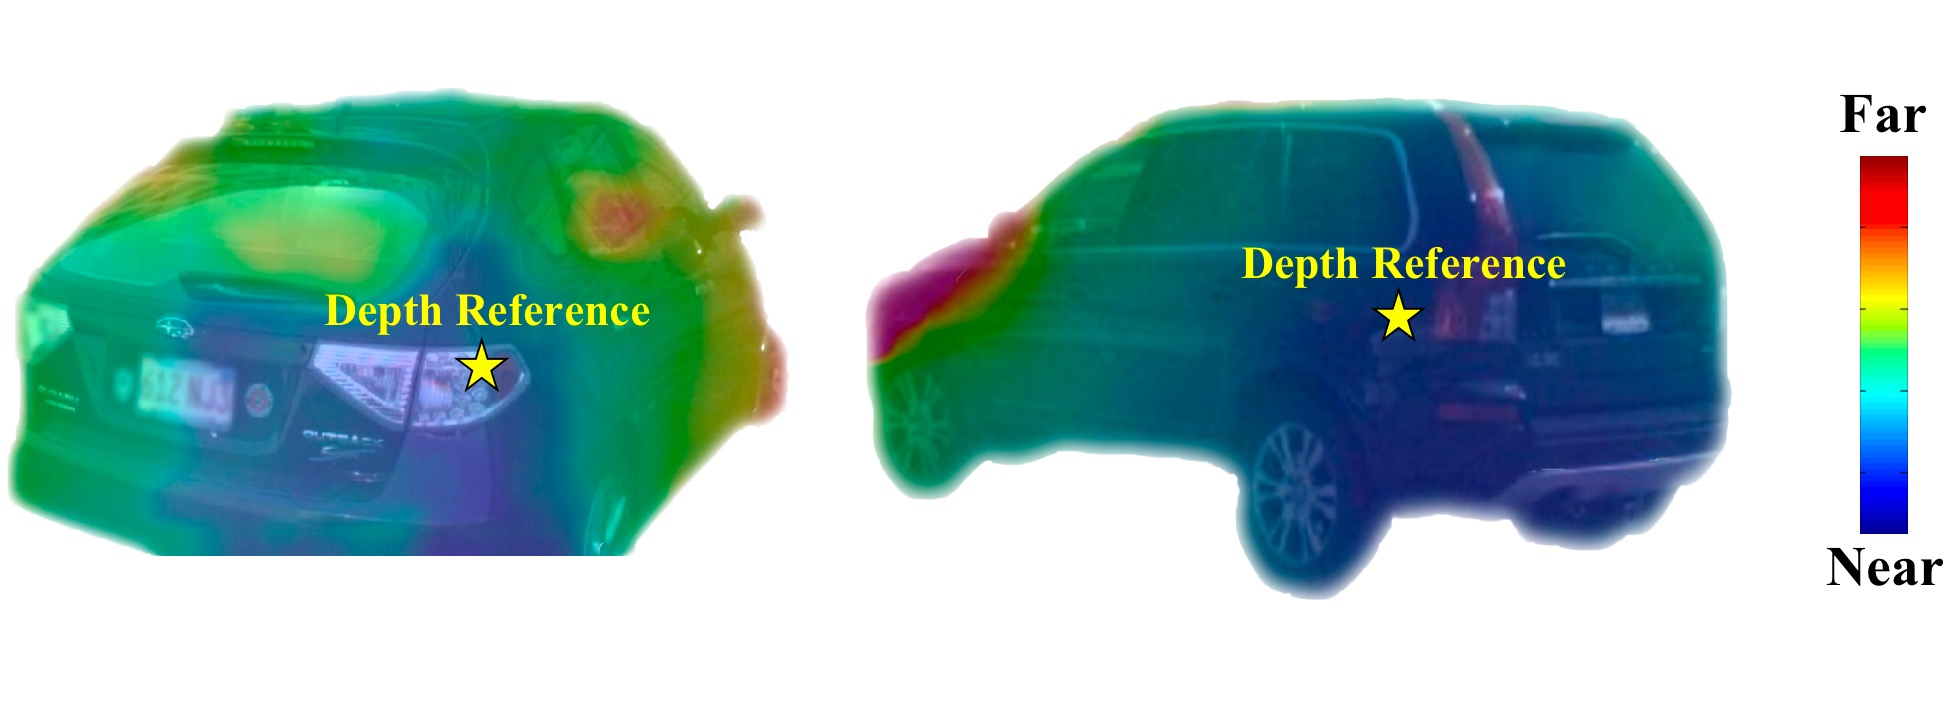
\includegraphics[scale=0.12]{cvpr_2022/depthref.jpeg}
    \caption{\textbf{Inner-depth Supervision.} We guide the camera-based detector to learn the relative spatial structures within the target foreground areas. A depth reference point (dotted in yellow) is adaptively selected to calculate relative depth values.}
    \label{fig:fig2}
    % \vspace{-0.8cm}
\end{figure}

To alleviate this issue, we propose a novel LiDAR-to-camera learning scheme, \textbf{TiG-BEV}, which involves the inner-geometry of foreground targets into the camera-based detectors for multi-view BEV 3D object detection. As shown in Figure~\ref{fig:teaser_figure} (c), we conduct simultaneous target inner-geometry learning for dense depth prediction and BEV feature generation.
First, besides the previous absolute depth map prediction~\cite{b7,b51}, we introduce an inner-depth supervision module within pixels of different foreground targets. A reference depth point is adaptively selected for each target to obtain the relative depth relationships shown in Figure~\ref{fig:fig2}, which contributes to high-quality depth map prediction with better target structural understanding. Second, we propose an inner-feature BEV distillation module, which imitates the high-level foreground BEV semantics produced by a pre-trained LiDAR-based detector. Different from previous dense and strict feature distillation~\cite{b9,b52}, we sample several keypoints within each BEV foreground area and guide the camera-based detector to learn their inner feature-similarities shown in Figure~\ref{fig:fig3}, which are in both inter-channel and inter-keypoint manners. In this way, the camera-based detector can not only inherit the high-level part-wise LiDAR semantics, but also relieve the modal gap by avoiding the strict feature mimicking. Through extensive experiments, we observe consistent performance improvement brought by TiG-BEV upon the baseline models. On nuScenes~\cite{b6} val set with equivalent settings, the powerful BEVDepth~\cite{b7} can be boosted by \textbf{+2.3\%} NDS and \textbf{+2.4\%} mAP, and BEVDet~\cite{b19} without CBGS can be further enhanced by \textbf{+9.1\%} NDS and \textbf{+10.3\%} mAP for BEVDet without CBGS, which well demonstrates the significance of our TiG-BEV.

The contributions of TiG-BEV are summarized below:
\begin{itemize}[leftmargin=*,itemsep=0pt,topsep=0pt]
    \item We introduce an inner-depth supervision module to model the relative depth relations of foreground targets, which leads to better depth map prediction.
    \item We propose an inner-feature BEV distillation module to transfer the well-learned knowledge from LiDAR modality to camera-based BEV representations. 
    \item Extensive experiments have verified the effectiveness of our approach to enhance the capacity for multi-view BEV 3D object detection.
\end{itemize}
\begin{figure}[!t]
% \vspace{-0.5cm}
    \centering
    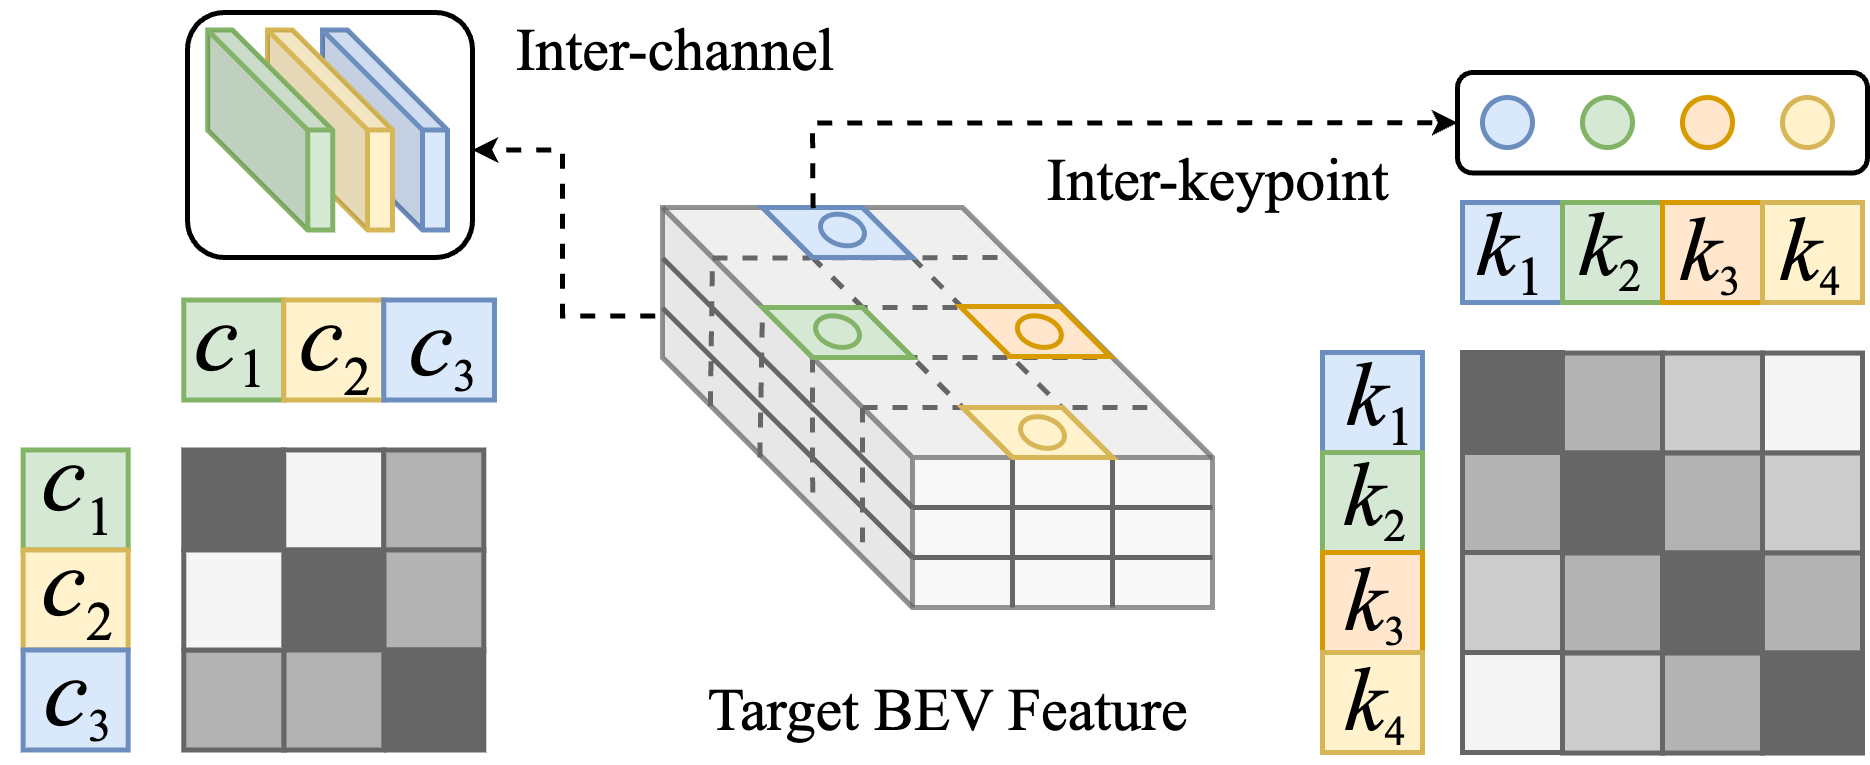
\includegraphics[scale=0.115]{cvpr_2022/iccv_fig3.drawio.png}
    \caption{\textbf{Inner-feature BEV Distillation.} We respectively conduct inter-channel and inter-keypoint feature distillation in BEV space for the camera-based detector, which alleviates the cross-modal semantic gap and boosts inner-geometry learning.}
    \label{fig:fig3}
    % \vspace{-0.8cm}
\end{figure}